% compile with: pdflatex -shell-escape filename.tex
\documentclass[crop,tikz,convert=pdf2svg]{standalone}
\usetikzlibrary{arrows.meta}
\usetikzlibrary{backgrounds}

\begin{document}

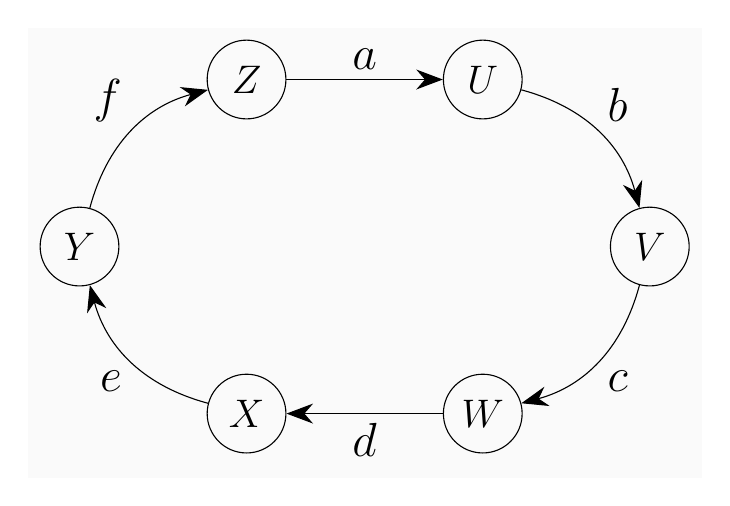
\begin{tikzpicture}[
    background rectangle/.style={fill=black!02},
    show background rectangle,
    -{Stealth[scale=2]},
    node distance=3cm,
    main node/.style={circle,draw,font=\sffamily\Large\bfseries,minimum size=1cm},
  ]

  \node[main node] (U) {$U$};
  \node[main node] (V) [below right of=U] {$V$};
  \node[main node] (W) [below left of=V] {$W$};
  \node[main node] (X) [left of=W] {$X$};
  \node[main node] (Y) [above left of=X] {$Y$};
  \node[main node] (Z) [above right of=Y] {$Z$};

  \path[every node/.style={font=\LARGE}]
  (U) edge [bend left] node[above right] {$b$}(V)
  (V) edge [bend left] node[below right] {$c$} (W)
  (W) edge node[below] {$d$} (X)
  (X) edge [bend left] node[below left] {$e$} (Y)
  (Y) edge [bend left] node[above left] {$f$} (Z)
  (Z) edge node[above] {$a$} (U)
  ;
\end{tikzpicture}
\end{document}
